\chapter{Biologie structurale des protéines}\label{ch:b3:structural-biology}

Max Perutz s'est attelé à la structure de l'hémoglobine en 1937 et l'a
publiée en 1960~: vingt-deux ans pour voir, à une \omterm{def:b3:structural-biology:methods}{résolution} d'un
demi-nanomètre, comment quatre chaînes de cent cinquante acides aminés
s'enroulent autour de quatre hèmes. Une molécule d'hémoglobine se
replie, elle, en quelques millisecondes. Entre ces deux faits se tient
le sujet de ce chapitre~: ce qu'est la forme d'une protéine, pourquoi
une chaîne d'acides aminés prend telle forme plutôt qu'une autre,
comment elle la trouve si vite parmi un nombre astronomique de
solutions, ce qui va de travers lorsqu'elle ne la trouve pas, comment
on voit ces formes --- par les rayons X, par la résonance magnétique,
par les électrons et, désormais, par le calcul --- et comment une
protéine passe d'une forme à l'autre pour faire son travail, la
bascule de l'hémoglobine entre une forme tendue et une forme relâchée
servant de modèle à toute protéine allostérique depuis lors.

\section{Ce qu'est la structure d'une protéine}

\begin{definition}[Les niveaux de structure]\label{def:b3:structural-biology:levels}
\index{structure secondaire}\index{hélice alpha}\index{feuillet bêta}\index{structure tertiaire}\index{domaine}\index{repliement}
La \emph{structure primaire} est la suite des résidus. La
\emph{structure secondaire} est la conformation régulière locale du
squelette, stabilisée par des liaisons hydrogène entre les carbonyles
et les amides du squelette~: l'\emph{hélice $\alpha$}, spirale droite
de $3.6$ résidus par tour, qui monte de \qty{0.15}{nm} par résidu
(\qty{0.54}{nm} par tour), chaque carbonyle étant lié à l'amide situé
quatre résidus plus loin~; et le \emph{feuillet $\beta$}, où des brins
étendus se rangent côte à côte, parallèles ou antiparallèles, liés à
leurs voisins, les chaînes latérales alternant au-dessus et au-dessous
du feuillet. La \emph{structure tertiaire} est le repliement d'une
chaîne entière dans l'espace~; une unité compacte qui s'y replie de
façon autonome, de \numrange{50}{250} résidus, est un \emph{domaine},
et l'agencement des éléments secondaires d'un domaine en est le
\emph{repliement}. La \emph{structure quaternaire} est l'assemblage de
plusieurs chaînes~: l'$\alpha_{2}\beta_{2}$ de l'hémoglobine. Environ
\num{1300} repliements rendent compte de tous les domaines connus, et
quelques dizaines d'entre eux --- le repliement de Rossmann, le
tonneau TIM, le repliement des immunoglobulines --- d'une grande part
de toutes les protéines~: la nature réemploie les repliements et varie
leurs séquences.
\end{definition}

\begin{omfigure}
\begin{tikzpicture}
\begin{axis}[
  width=6.4cm, height=6.4cm,
  xmin=-180, xmax=180, ymin=-180, ymax=180,
  xlabel={$\phi$ (degrés)}, ylabel={$\psi$ (degrés)},
  xlabel style={font=\small}, ylabel style={font=\small},
  tick label style={font=\scriptsize}, xtick={-180,-90,0,90,180}, ytick={-180,-90,0,90,180},
  axis lines=box, grid=major, grid style={gray!25},
  clip=false,
]
% beta region
\fill[omDef!30] (axis cs:-180,90) rectangle (axis cs:-45,180);
\fill[omDef!30] (axis cs:-180,-180) rectangle (axis cs:-45,-150);
\node[font=\scriptsize, omDef!60!black] at (axis cs:-112,165) {brins $\beta$};
% alpha R region
\fill[omThm!30] (axis cs:-160,-70) rectangle (axis cs:-45,0);
\node[font=\scriptsize, omThm!70!black] at (axis cs:-105,-58) {$\alpha$ droite};
% alpha L region
\fill[omMeth!30] (axis cs:45,0) rectangle (axis cs:100,80);
\node[font=\scriptsize, omMeth!60!black, align=center] at (axis cs:72,40) {hélice\\gauche};
\addplot[only marks, mark=*, mark size=1pt, black] coordinates {(-57,-47)};
\node[font=\scriptsize, anchor=south west] at (axis cs:-52,-44) {$\alpha$: $(-57,-47)$};
\addplot[only marks, mark=*, mark size=1pt, black] coordinates {(-139,135)};
\node[font=\scriptsize, anchor=west] at (axis cs:-134,135) {$\beta$ antiparallèle};
\end{axis}
\node[align=left, font=\scriptsize, anchor=west] at (7.0,3.0) {Les deux angles de torsion du squelette de chaque\\résidu, $\phi$ (autour de N--C$_\alpha$) et $\psi$ (autour de\\C$_\alpha$--C), sont restreints par les encombrements\\aux régions colorées. Une hélice met chaque résidu\\en un même point~; un brin, près d'un autre. La\\glycine, sans chaîne latérale, va plus loin~; la\\proline, avec son cycle, est fixée près de $\phi = -60$.};
\end{tikzpicture}

{\small Le diagramme de Ramachandran. Les régions grisées sont les
combinaisons des angles de squelette $\phi$ et $\psi$ permises par
l'encombrement stérique~; l'hélice $\alpha$ droite et le brin $\beta$
correspondent chacun à une petite région, et la plupart des résidus
d'une protéine repliée tombent dans l'une d'elles.}
\end{omfigure}

\begin{proposition}[Ce qui tient un repliement]\label{prop:b3:structural-biology:forces}
\index{effet hydrophobe}\index{stabilité marginale}
Une protéine repliée est stabilisée par l'\emph{\omterm{prop:b3:structural-biology:forces}{effet hydrophobe}} ---
enfouir les chaînes latérales apolaires dans un cœur à l'abri de l'eau,
ce qui libère les molécules d'eau qui seraient sinon ordonnées autour
d'elles --- par les liaisons hydrogène de la \omterm{def:b3:structural-biology:levels}{structure secondaire} et
des groupements polaires enfouis, par l'empilement de van der Waals
d'un cœur aussi dense qu'un cristal, par quelques ponts salins et, dans
les protéines sécrétées, par des ponts disulfure. L'\omterm{prop:b3:structural-biology:forces}{effet hydrophobe}
fournit l'essentiel du moteur~; les liaisons hydrogène se paient pour
l'essentiel elles-mêmes (un squelette lié à l'eau à l'état déplié est
lié à lui-même à l'état replié) et dictent plutôt \emph{quel}
\omterm{def:b3:structural-biology:levels}{repliement}. L'énergie libre nette du \omterm{def:b3:structural-biology:levels}{repliement} est faible,
$\Delta G \approx -20$ à \qty{-60}{kJ/mol} --- la force d'une poignée
de liaisons hydrogène pour une molécule qui en compte des centaines ---
parce que la perte d'entropie conformationnelle au \omterm{def:b3:structural-biology:levels}{repliement} annule
presque le gain d'enthalpie. Les protéines sont de
\emph{\omterm{prop:b3:structural-biology:forces}{stabilité marginale}}~: quelques degrés, un changement de pH, une
seule mutation dans le cœur peuvent les déplier, et cette marginalité
est ce qui leur permet de bouger.
\end{proposition}

\begin{proof}[Faits expérimentaux]
Anfinsen (1961) a déplié la ribonucléase~A par l'urée et un réducteur,
rompant ses quatre ponts disulfure et détruisant son activité~; en
retirant l'un et l'autre, l'enzyme s'est repliée de nouveau, a reformé
les quatre bons appariements disulfure parmi les $105$ possibles et a
retrouvé toute son activité. Aucune matrice, aucune enzyme, aucune
information au-delà de la séquence n'était présente~: la structure
native est l'état thermodynamiquement le plus stable accessible à la
chaîne, et la séquence l'encode. Réoxyder les ponts disulfure alors que
la chaîne était encore dans l'urée donnait un mélange brouillé à
\qty{1}{\%} d'activité, qui se démêlait ensuite vers la forme native
dès qu'on laissait la chaîne se replier~: la chaîne trouve le minimum
toute seule.
\end{proof}

\section{Comment une chaîne trouve son repliement}

\begin{theorem}[Le paradoxe de Levinthal]\label{thm:b3:structural-biology:levinthal}
\index{paradoxe de Levinthal}\index{entonnoir de repliement}
Si chacun des $n$ résidus d'une protéine pouvait prendre $k$
conformations de squelette indépendamment, la chaîne aurait $k^{n}$
conformations. Avec $k = 3$ et $n = 100$ cela fait $3^{100} \approx
5\times 10^{47}$~; les échantillonner à raison d'une par picoseconde
($10^{12}$ par seconde) prendrait $5\times 10^{35}$ secondes, soit
environ $10^{28}$ ans. Les protéines de cette taille se replient en
quelques millisecondes à quelques secondes. Le \omterm{def:b3:structural-biology:levels}{repliement} n'est donc
pas une recherche au hasard parmi les conformations~: la surface
d'énergie est un \emph{entonnoir}, où presque toute conformation
partielle est biaisée vers l'état natif, et la chaîne y descend par des
mouvements locaux qui vont chacun, en moyenne, vers le bas.
\end{theorem}
\begin{proof}
Le dénombrement est le principe multiplicatif~; le temps est ce compte
divisé par la cadence d'échantillonnage,
$5\times 10^{47}/10^{12} = 5\times
10^{35}$ s, et une année fait $3\times 10^{7}$ s. La conclusion est la
contraposée~: une recherche au hasard de cette taille est impossible
dans le temps observé, donc la recherche n'est pas au hasard. Ce qui la
rend non aléatoire est qu'une interaction formée dans une partie de la
chaîne persiste pendant que d'autres se forment (l'effondrement
hydrophobe et la formation des hélices prennent des microsecondes et
réduisent l'espace à explorer), et que des structures partiellement
justes sont en moyenne d'énergie plus basse que des structures fausses,
de sorte que la descente est guidée --- un entonnoir plutôt qu'un
terrain de golf percé d'un seul trou.
\end{proof}

\begin{omfigure}
\begin{tikzpicture}[every node/.style={font=\scriptsize}, >=stealth]
  % funnel outline
  \draw[very thick, omDef] (-4,3) .. controls (-3.2,1.5) and (-1.2,0.2) .. (-0.35,-1.2) -- (-0.35,-1.6);
  \draw[very thick, omDef] (4,3) .. controls (3.2,1.5) and (1.2,0.2) .. (0.35,-1.2) -- (0.35,-1.6);
  \draw[very thick, omDef] (-0.35,-1.6) -- (0.35,-1.6);
  % rugged inner lines
  \draw[omDef!60, thick] (-3.3,2.6) .. controls (-2.9,2.2) and (-2.6,2.6) .. (-2.2,2.0) .. controls (-1.9,1.5) and (-1.7,1.9) .. (-1.4,1.2) .. controls (-1.1,0.7) and (-0.9,0.9) .. (-0.6,0.2);
  \draw[omDef!60, thick] (3.3,2.6) .. controls (2.9,2.1) and (2.5,2.5) .. (2.1,1.8) .. controls (1.8,1.3) and (1.5,1.6) .. (1.2,1.0) .. controls (1.0,0.6) and (0.8,0.8) .. (0.6,0.2);
  % axes
  \draw[->] (-5.9,-1.8) -- (-5.9,3.2) node[above, align=center] {énergie\\libre};
  \draw[<->] (-3.9,3.85) -- (3.9,3.85) node[midway, above] {entropie conformationnelle (largeur de l'ensemble)};
  % labels
  \node[above] at (0,3.05) {chaîne dépliée~: de nombreuses conformations, énergie élevée};
  \node[right, align=left] at (3.3,1.4) {pièges locaux~: intermédiaires\\partiellement mal repliés};
  \node[left, align=right] at (-3.3,1.4) {effondrement rapide et\\structure secondaire};
  \node[below] at (0,-1.7) {état natif~: une seule conformation, énergie la plus basse};
  \draw[->, thick, omThm] (-2.8,2.4) .. controls (-2.0,1.2) and (-0.8,0.5) .. (-0.15,-1.3);
  \node[omThm, left] at (-1.5,-0.5) {une trajectoire de repliement};
\end{tikzpicture}

{\small L'\omterm{thm:b3:structural-biology:levinthal}{entonnoir de repliement}. L'énergie libre diminue et le nombre
de conformations accessibles se réduit à mesure que la chaîne approche
de l'état natif~; les parois sont accidentées, de sorte qu'une chaîne
peut se trouver piégée dans un intermédiaire mal replié, mais la pente
d'ensemble l'entraîne vers le bas en quelques millisecondes.}
\end{omfigure}

\begin{definition}[Les chaperons]\label{def:b3:structural-biology:chaperones}
\index{chaperon}\index{Hsp70}\index{chaperonine}\index{GroEL}
Un \emph{chaperon moléculaire} est une protéine qui assiste le
\omterm{def:b3:structural-biology:levels}{repliement} des autres sans entrer dans leur composition ni fournir
d'information sur le \omterm{def:b3:structural-biology:levels}{repliement}~: il empêche l'agrégation qui concurrence
le \omterm{def:b3:structural-biology:levels}{repliement} dans un cytoplasme encombré. \emph{Hsp70} se fixe sur les
segments hydrophobes exposés des chaînes naissantes ou dépliées et les
relâche à l'hydrolyse de l'ATP pour une nouvelle tentative~; la
\emph{chaperonine} GroEL (Hsp60 dans les mitochondries, TRiC dans le
cytosol eucaryote) est un double tonneau de quatorze sous-unités dont
la cavité centrale, coiffée par GroES, enferme à l'écart une chaîne
unique allant jusqu'à \qty{60}{kDa} pendant une dizaine de secondes ---
une cage d'Anfinsen --- et l'éjecte repliée ou non, pour un nouvel
essai. Environ un dixième des protéines bactériennes néosynthétisées
passe par GroEL, et une cellule dont les chaperons sont débordés ---
par la chaleur, ce qui explique que la plupart soient des
\emph{protéines de choc thermique} induites par une élévation de
température --- se remplit d'agrégats.
\end{definition}

\begin{definition}[L'amyloïde]\label{def:b3:structural-biology:amyloid}
\index{amyloïde}\index{croisé-bêta}\index{prion}\index{maladie du mauvais repliement}
Une \emph{amyloïde} est un agrégat ordonné de protéines où les chaînes
s'empilent en fibrilles non ramifiées de \qtyrange{5}{10}{nm} de large,
les brins de chaque chaîne courant perpendiculairement à l'axe de la
fibrille et liés par hydrogène aux brins de la suivante --- la
structure \emph{croisée-$\beta$}, la même quelle que soit la protéine.
Presque toute protéine peut la former dans des conditions
déstabilisantes~; dans les \emph{maladies du mauvais \omterm{def:b3:structural-biology:levels}{repliement}},
certaines protéines le font dans l'organisme~: l'amyloïde-$\beta$ et
tau dans la maladie d'Alzheimer, l'$\alpha$-synucléine dans celle de
Parkinson, la huntingtine, la transthyrétine, l'amyloïde des îlots dans
le diabète de type~2. Un \emph{prion} est une amyloïde qui se
propage~: la forme mal repliée de la protéine prion PrP convertit au
contact la forme normale en une copie d'elle-même, de sorte que
l'«~infection~» ne transporte aucun acide nucléique, seulement une
forme --- le mécanisme de la tremblante du mouton, de
l'encéphalopathie spongiforme bovine et de la maladie de
Creutzfeldt--Jakob, établi par Prusiner à partir de 1982 contre une
longue résistance.
\end{definition}

\begin{omfigure}
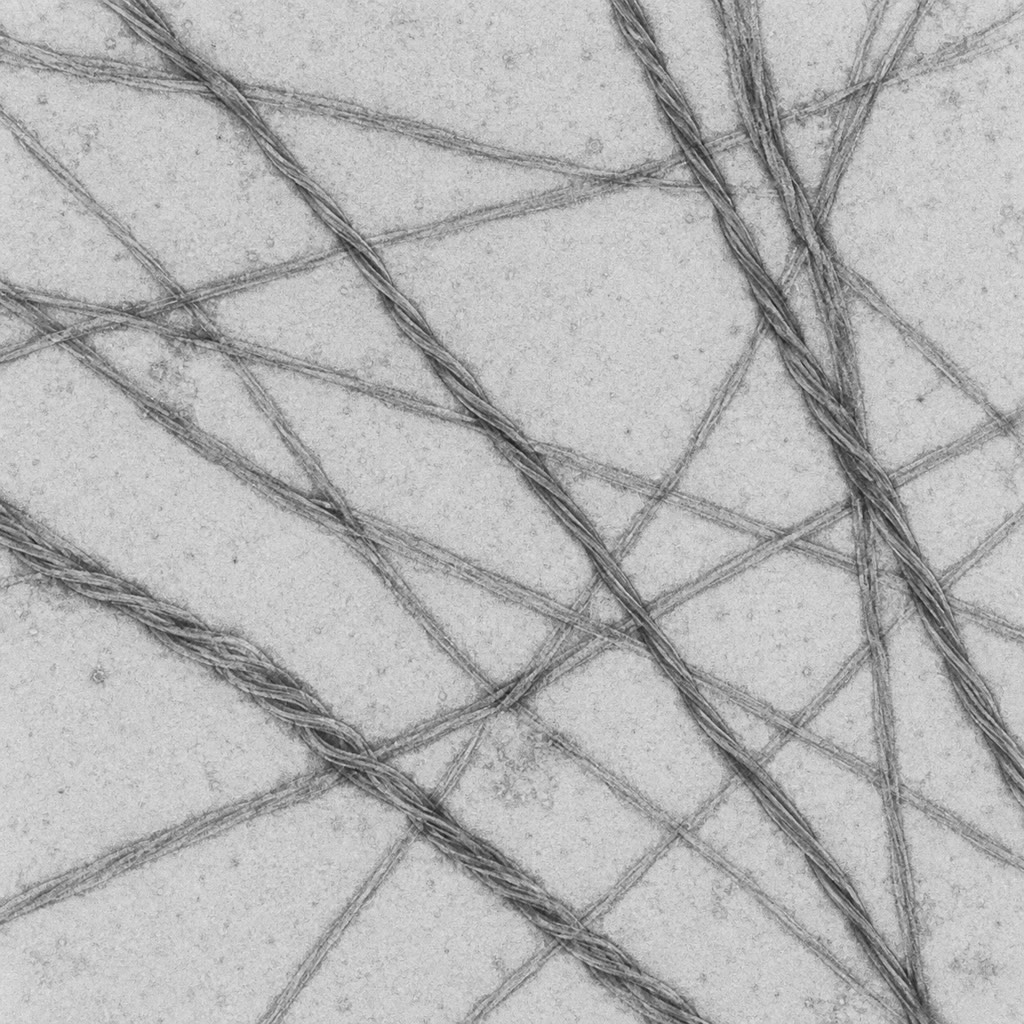
\includegraphics[width=0.36\linewidth]{images/book5/ai/b5-07-amyloid-fibrils.jpg}\hspace{0.04\linewidth}
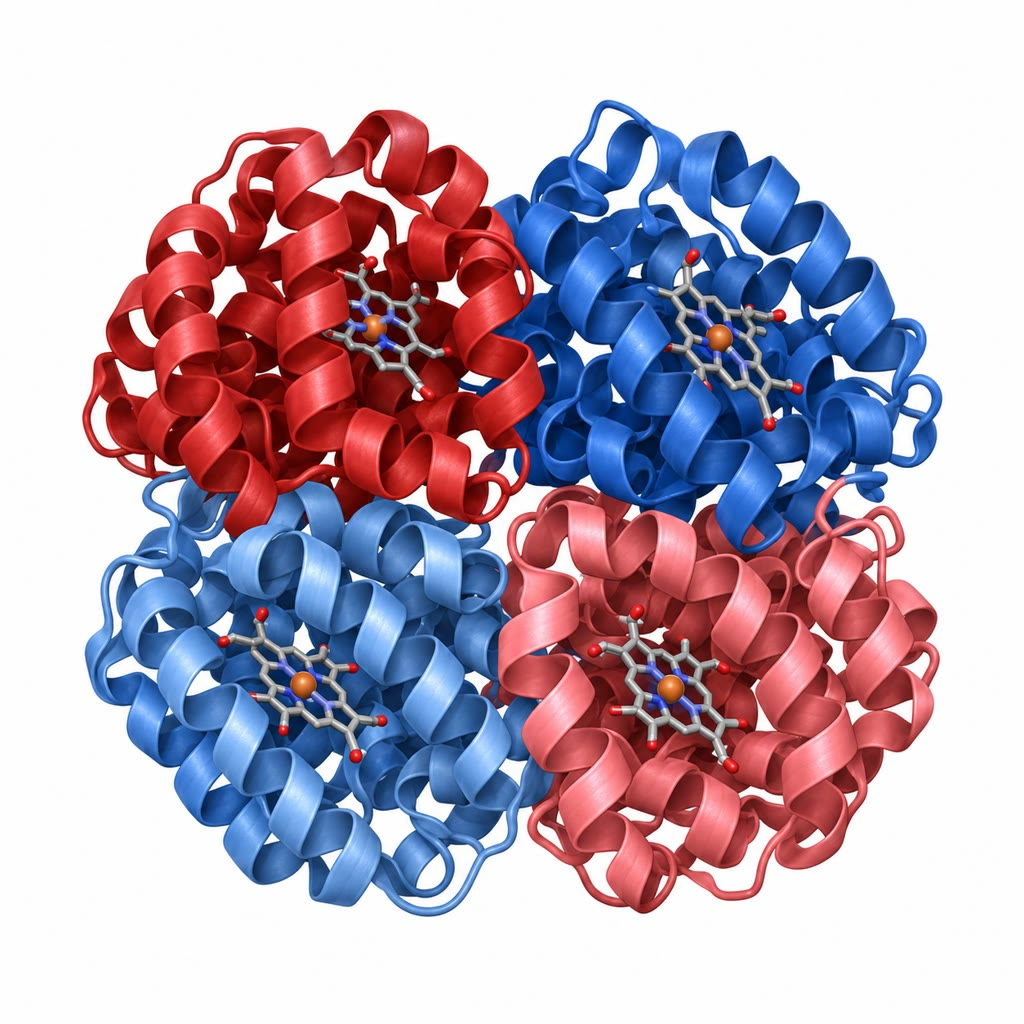
\includegraphics[width=0.36\linewidth]{images/book5/ai/b5-07-haemoglobin-model.jpg}

{\small À gauche~: des fibrilles \omterm{def:b3:structural-biology:amyloid}{amyloïdes} au microscope électronique
--- droites, non ramifiées, parfois torsadées, et semblables quelle que
soit la protéine dont elles sont faites. À droite~: le tétramère
d'hémoglobine, deux chaînes $\alpha$ et deux chaînes $\beta$, chacune
berçant un hème.}
\end{omfigure}

\section{Voir une protéine}

\begin{definition}[Les méthodes structurales]\label{def:b3:structural-biology:methods}
\index{cristallographie aux rayons X}\index{spectroscopie RMN}\index{cryomicroscopie électronique}\index{résolution}
La \emph{cristallographie aux rayons X} fait croître un cristal de la
protéine, l'expose à un faisceau de rayons X et enregistre la figure de
diffraction~; la position des taches donne le réseau et leurs
intensités, une fois les phases des ondes retrouvées, donnent la
densité électronique de la maille, dans laquelle la chaîne est
construite. La \emph{résonance magnétique nucléaire} (RMN) mesure, en
solution, les couplages entre les noyaux d'atomes proches dans
l'espace, d'où l'on calcule des distances puis une structure~; elle
fonctionne pour des protéines de moins de \qty{40}{kDa} environ et rend
compte de leurs mouvements. La \emph{cryomicroscopie électronique}
image des milliers à des millions de molécules isolées, congelées dans
un film mince de glace vitreuse, chacune dans une orientation au
hasard, et reconstruit la densité tridimensionnelle en les combinant~;
depuis les détecteurs d'électrons directs (2013) elle atteint la
résolution atomique et n'exige aucun cristal, de sorte que de grands
complexes, des protéines membranaires et des assemblages souples qui
n'ont jamais cristallisé se résolvent aujourd'hui couramment. La
\emph{résolution} d'une structure est le plus petit écart auquel deux
détails restent séparés~: à \qty{0.35}{nm} on place le squelette et les
grandes chaînes latérales, à \qty{0.2}{nm} chaque atome, à
\qty{0.1}{nm} les hydrogènes.
\end{definition}

\begin{proof}[Faits expérimentaux]
Kendrew (1958) a obtenu la première structure d'une protéine, la
myoglobine de cachalot, à \qty{0.6}{nm} --- un boudin d'une
irrégularité inattendue, «~plus compliqué et moins symétrique que
quiconque l'avait prédit~» --- puis à \qty{0.2}{nm} en 1960, lorsque
les hélices $\alpha$ que Pauling avait proposées par construction de
modèles en 1951 furent vues pour la première fois. Perutz (1960) a
résolu l'hémoglobine à \qty{0.55}{nm} par la méthode des atomes lourds
qu'il avait imaginée pour obtenir les phases~: des atomes de mercure
fixés à la protéine changent les intensités d'une manière qui révèle
l'information manquante. En comparant les formes oxygénée et
désoxygénée (1970), il a vu les sous-unités tourner les unes contre les
autres de \qty{15}{\degree} à la fixation du dioxygène, première
transition allostérique observée à l'échelle atomique.
\end{proof}

\begin{omfigure}
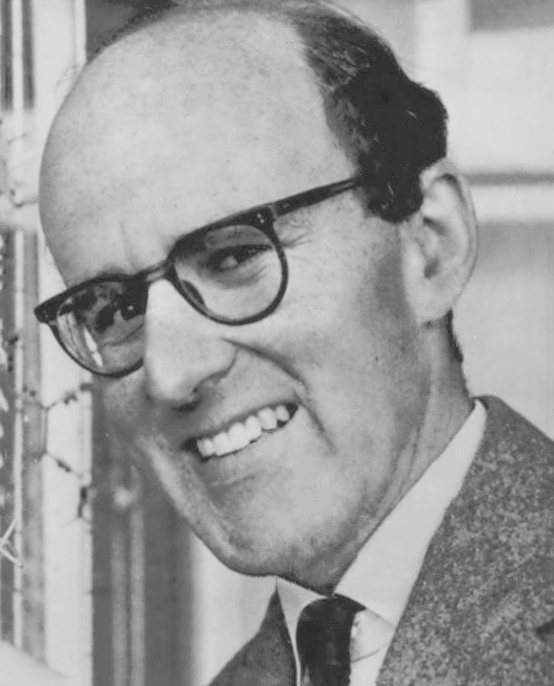
\includegraphics[width=0.30\linewidth]{images/book5/perutz.jpg}\hspace{0.04\linewidth}
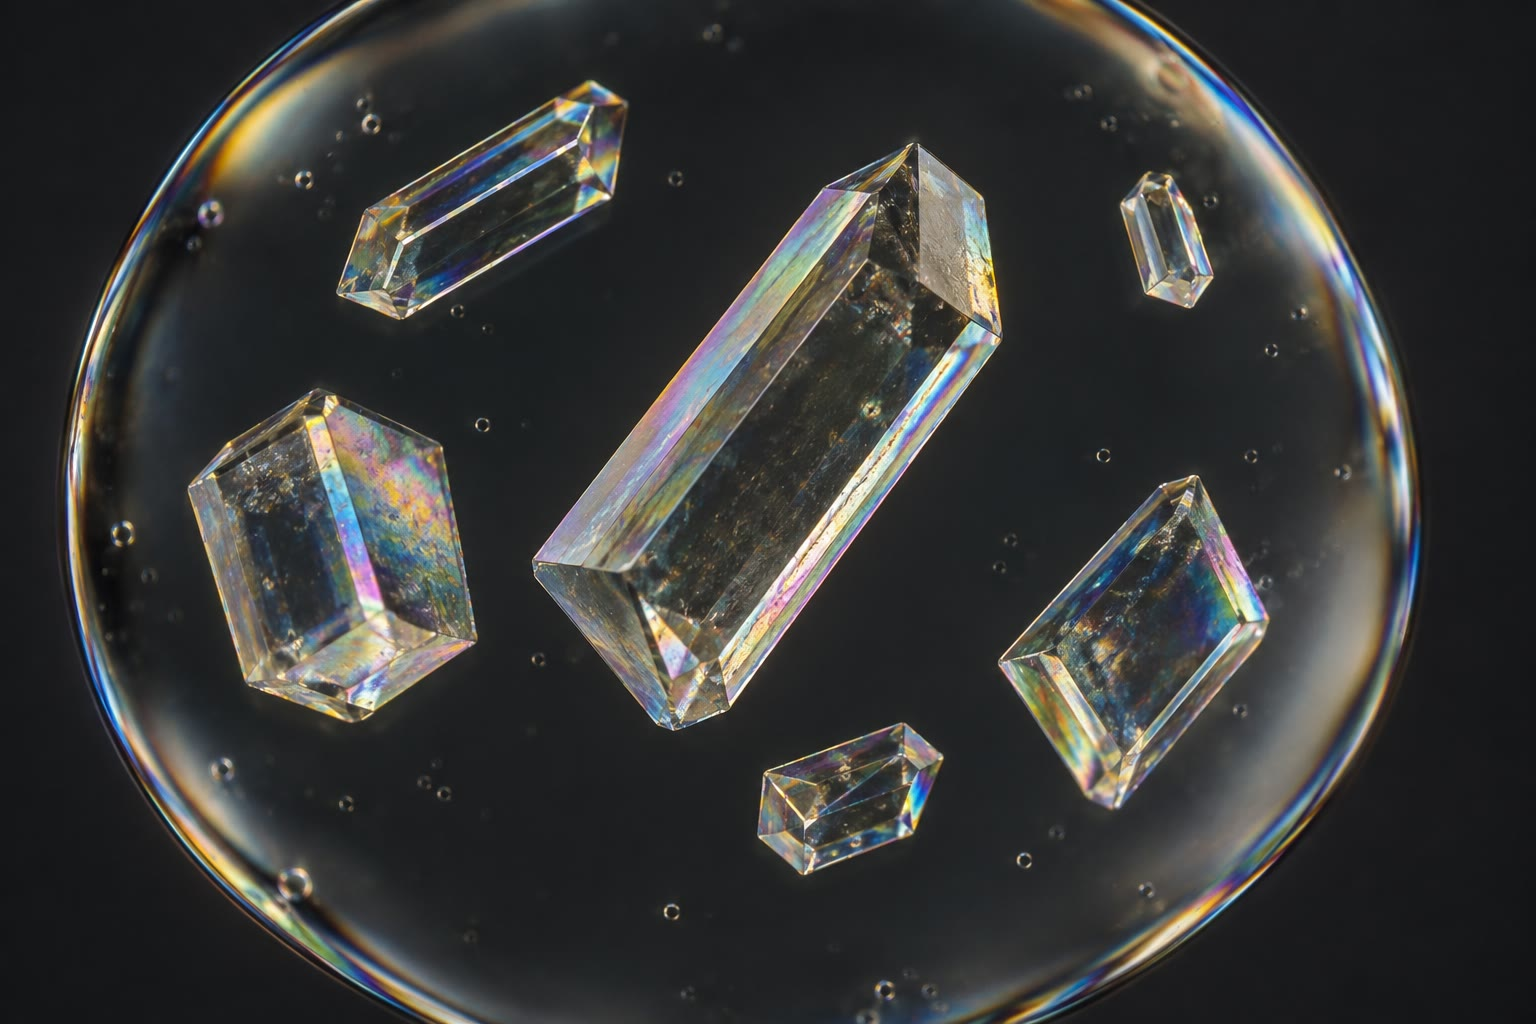
\includegraphics[width=0.30\linewidth]{images/book5/ai/b5-07-protein-crystals.jpg}\hspace{0.04\linewidth}
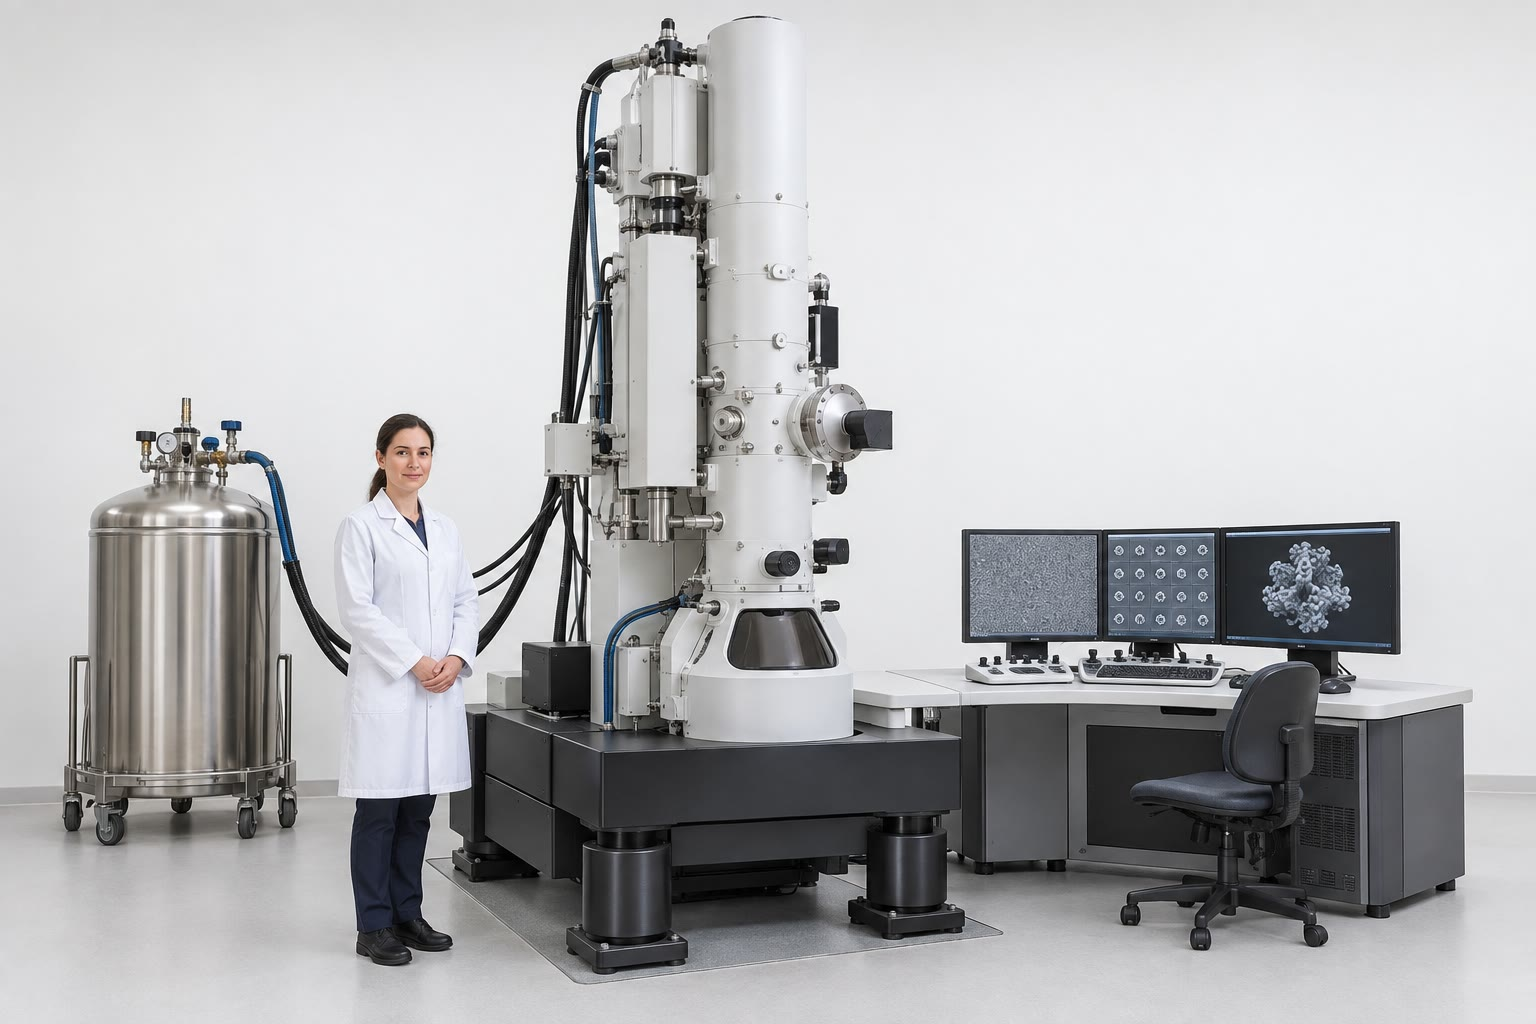
\includegraphics[width=0.30\linewidth]{images/book5/ai/b5-07-cryo-em.jpg}

{\small Max Perutz en 1962, l'année de son prix Nobel pour la structure
de l'hémoglobine (Associated Press, \omterm{def:b3:structural-biology:levels}{domaine} public). Au centre~: des
cristaux de protéine dans une goutte suspendue, point de départ de la
cristallographie. À droite~: un cryomicroscope électronique,
l'instrument qui a rendu les cristaux inutiles.}
\end{omfigure}

\begin{method}[Résoudre une structure par cristallographie]\label{met:b3:structural-biology:crystallography}
\index{loi de Bragg}\index{problème des phases}
(1) Purifier des milligrammes de la protéine et cribler des centaines
de conditions (précipitant, pH, sel) pour obtenir des cristaux~;
(2) congeler brusquement un cristal et collecter les clichés de
diffraction à un synchrotron pendant qu'il tourne dans le faisceau~;
(3) indexer les taches pour obtenir la maille et la symétrie~; l'angle
le plus grand auquel on voit des taches fixe la \omterm{def:b3:structural-biology:methods}{résolution} par la \omterm{met:b3:structural-biology:crystallography}{loi
de Bragg}, $d =
\lambda/(2\sin\theta)$~; (4) résoudre le \emph{\omterm{met:b3:structural-biology:crystallography}{problème des phases}} ---
le détecteur enregistre des intensités mais non des phases --- par des
atomes lourds, par la diffusion anomale du sélénium de la
sélénométhionine, ou, pour une protéine voisine d'une protéine connue,
par remplacement moléculaire, en plaçant le modèle connu dans la
maille~; (5) calculer la densité électronique, y construire la chaîne
et affiner le modèle contre les données jusqu'à ce que le désaccord
(facteur $R$) soit petit~; (6) valider~: géométrie, écarts au
diagramme de Ramachandran, et accord avec des données contre
lesquelles le modèle n'a pas été affiné.
\end{method}

\begin{omfigure}
\begin{tikzpicture}[every node/.style={font=\scriptsize}, >=stealth]
  % crystal
  \draw[thick, fill=omDef!20] (0,0) -- (1.4,0) -- (1.9,0.6) -- (0.5,0.6) -- cycle; \draw[thick, fill=omDef!30] (0,0) -- (0.5,0.6) -- (0.5,1.6) -- (0,1.0) -- cycle; \draw[thick, fill=omDef!25] (0.5,0.6) -- (1.9,0.6) -- (1.9,1.6) -- (0.5,1.6) -- cycle;
  \node[below] at (0.95,-0.1) {cristal~: $10^{12}$ molécules en registre};
  % beam
  \draw[->, very thick, omThm] (-2.2,0.9) -- (-0.1,0.9); \node[above] at (-1.2,0.95) {rayons X, $\lambda \approx \qty{0.1}{nm}$};
  % diffracted beams
  \foreach \a in {-25,-12,5,18,30} \draw[->, omThm, thick] (1.9,0.9) -- ++(\a:3.2);
  % detector
  \draw[thick] (5.2,-1.2) rectangle (5.6,3.0); \node[right, align=left] at (5.7,2.6) {détecteur~: taches aux\\angles $\theta$, d'intensités $I$};
  \foreach \y in {-0.6,-0.1,0.6,1.2,1.9,2.4} \fill[black] (5.4,\y) circle (0.06);
  % arrow to density
  \draw[->, very thick] (7.4,0.9) -- (8.6,0.9) node[midway, above, align=center] {phases\\retrouvées};
  \node[right, align=left] at (8.7,1.4) {densité électronique};
  \draw[omDef, thick] (8.8,0.4) .. controls (9.1,1.1) and (9.5,0.2) .. (9.8,0.8) .. controls (10.1,1.3) and (10.4,0.3) .. (10.7,0.9);
  \node[right, align=left] at (8.7,-0.4) {modèle construit dedans,\\affiné, validé};
  % Bragg
  \node[anchor=north west, align=left] at (-2.2,-0.7) {Bragg~: $2d\sin\theta = \lambda$ ---\\le plus grand $\theta$ observé fixe la résolution $d$};
\end{tikzpicture}

{\small Du cristal au modèle. Le réseau régulier diffracte les rayons X
en taches discrètes~; la tache de plus grand angle fixe la \omterm{def:b3:structural-biology:methods}{résolution}~;
retrouver les phases transforme les intensités en une carte de densité
électronique, dans laquelle la chaîne est construite.}
\end{omfigure}

\begin{remark}[La prédiction a rejoint les méthodes]\label{rem:b3:structural-biology:prediction}
Depuis 2020, la structure d'une protéine se prédit à partir de sa
séquence avec une exactitude qui rivalise souvent avec une structure
expérimentale à \qty{0.3}{nm} (\cref{ch:b3:bioinformatics}). La
prédiction est une hypothèse sur un état natif statique~; les méthodes
expérimentales restent l'arbitre, et la seule source d'information sur
les ligands, les changements de conformation, les complexes et la
dynamique dont il est question plus bas. Leurs rôles ont changé --- un
modèle prédit résout le \omterm{met:b3:structural-biology:crystallography}{problème des phases} par remplacement
moléculaire, et oriente les expériences qui valent la peine --- plutôt
que l'un ne remplace l'autre.
\end{remark}

\section{L'allostérie~: l'hémoglobine pour modèle}

\begin{definition}[Allostérie et coopérativité]\label{def:b3:structural-biology:allostery}
\index{allostérie}\index{coopérativité}\index{coefficient de Hill}\index{état T}\index{état R}
Une protéine est \emph{allostérique} lorsque la fixation d'un ligand
sur un site change l'affinité d'un autre site, par un changement de
conformation transmis à travers la molécule. Lorsque les deux sites
fixent le même ligand et que l'effet est positif, la fixation est
\emph{coopérative}~: la saturation fractionnaire $Y$ croît avec la
concentration du ligand en sigmoïde et non en hyperbole, ce que décrit
empiriquement l'\emph{équation de Hill} $Y = [S]^{n_{H}}/(K^{n_{H}} +
[S]^{n_{H}})$ avec un \emph{coefficient de Hill} $n_{H} > 1$
(hémoglobine~: $n_{H} \approx 2.8$ pour ses quatre sites~; myoglobine,
un seul site~: $n_{H} =
1$). L'hémoglobine existe en deux conformations quaternaires,
l'\emph{état T} (tendu, de faible affinité, favorisé lorsque aucun
dioxygène n'est fixé) et l'\emph{état R} (relâché, de forte affinité),
et bascule de l'une à l'autre en bloc~; les protons, le dioxyde de
carbone et le 2,3-bisphosphoglycérate stabilisent T et abaissent donc
l'affinité --- c'est l'\omterm{prop:b3:structural-biology:mechanism}{effet Bohr}, par lequel un tissu au travail,
acide et chaud, prend davantage de dioxygène au sang.
\end{definition}

\begin{theorem}[Le modèle de Monod--Wyman--Changeux]\label{thm:b3:structural-biology:mwc}
\index{modèle de Monod--Wyman--Changeux}\index{modèle concerté}
Soit une protéine à $n$ sites identiques, existant en deux
conformations $T$ et $R$, en équilibre $L = [T_{0}]/[R_{0}]$ en
l'absence de ligand, chaque site de $R$ fixant le ligand avec la
constante de dissociation $K_{R}$ et chaque site de $T$ avec $K_{T}$,
$c = K_{R}/K_{T} < 1$. Tous les sites d'une molécule basculent ensemble
(la transition est \emph{concertée}). Alors, avec
$\alpha = [S]/K_{R}$, la saturation fractionnaire vaut
\[
Y = \frac{\alpha(1+\alpha)^{n-1} + Lc\alpha(1+c\alpha)^{n-1}}
{(1+\alpha)^{n} + L(1+c\alpha)^{n}},
\]
et la fraction de molécules à l'état $R$ vaut $\bar R =
(1+\alpha)^{n}/\bigl[(1+\alpha)^{n} + L(1+c\alpha)^{n}\bigr]$. Pour $L
\gg 1$ et $c \ll 1$ la courbe est sigmoïde~: les premiers ligands se
fixent sur les rares molécules $R$, de forte affinité, et font basculer
l'équilibre, de sorte que la fixation recrute davantage de $R$ et que
l'affinité des sites restants s'élève --- une \omterm{def:b3:structural-biology:allostery}{coopérativité} sans
aucune interaction directe entre sites.
\end{theorem}
\begin{proof}
L'espèce qui porte $i$ ligands sous la forme $R$ a pour concentration
$[R_{0}]\binom{n}{i}\alpha^{i}$ (chacun des $\binom{n}{i}$ choix de
sites occupés contribuant $([S]/K_{R})^{i}$ par la loi d'action de
masse), et sous la forme $T$ $[T_{0}]\binom{n}{i}(c\alpha)^{i}$,
puisque $[S]/K_{T} = c\alpha$. En sommant sur $i$ par la formule du
binôme, la protéine totale vaut
$[R_{0}]\bigl[(1+\alpha)^{n} + L(1+c\alpha)^{n}\bigr]$ et le ligand
total fixé vaut $[R_{0}]\sum_{i} i\binom{n}{i}\bigl[
\alpha^{i} + L(c\alpha)^{i}\bigr] = [R_{0}]\,n\bigl[\alpha(1+\alpha)^{n-1}
+ Lc\alpha(1+c\alpha)^{n-1}\bigr]$, d'après $\sum_{i} i\binom{n}{i}x^{i} =
nx(1+x)^{n-1}$. Diviser le ligand fixé par $n$ fois la protéine totale
donne $Y$~; la fraction $R$ est la somme des termes $R$ sur le total.
Lorsque $\alpha$ est petit, les termes $T$ dominent le dénominateur
(parce que $L \gg 1$) et $Y \approx c\alpha$, la faible affinité de
$T$~; lorsque $\alpha$ est assez grand pour que
$(1+\alpha)^{n} > L(1+c\alpha)^{n}$, les termes $R$ l'emportent et
l'affinité devient $K_{R}$~: la bascule entre les deux régimes est la
sigmoïde.
\end{proof}

\begin{example}[L'hémoglobine en chiffres]\label{ex:b3:structural-biology:hb-numbers}
Prenons $n = 4$, $K_{R} = \qty{1}{mmHg}$, $c = 0.01$ (donc $K_{T} =
\qty{100}{mmHg}$) et $L = 3\times 10^{5}$. À la pression partielle de
dioxygène du sang artériel, \qty{100}{mmHg}, $\alpha = 100$ et $Y =
0.97$~; à \qty{40}{mmHg}, la valeur veineuse au repos, $Y = 0.78$~; à
\qty{26}{mmHg}, $Y = 0.52$ --- le modèle reproduit la pression de
demi-saturation de \qty{26}{mmHg}~; à \qty{20}{mmHg}, dans un muscle à
l'exercice, $Y = 0.35$. Un transporteur non coopératif de même pression
de demi-saturation donnerait $100/126 = 0.79$ dans les poumons et
$20/46 = 0.43$ dans le muscle, cédant $0.36$ de sa capacité là où
l'hémoglobine en cède $0.62$. La \omterm{def:b3:structural-biology:allostery}{coopérativité} est ce qui fait un
transporteur qui se charge à fond à une pression et se décharge
largement à une pression cinq fois plus basse seulement.
\end{example}

\begin{omfigure}
\begin{tikzpicture}
\begin{axis}[
  width=0.7\linewidth, height=5.8cm,
  axis x line=bottom, axis y line=left,
  xmin=0, xmax=120, ymin=0, ymax=1.05,
  xlabel={pression partielle de dioxygène (mmHg)}, ylabel={saturation $Y$},
  xlabel style={font=\small, at={(axis description cs:0.5,-0.12)}, anchor=north},
  ylabel style={font=\small},
  tick label style={font=\small}, xtick={0,20,40,60,80,100,120}, ytick={0,0.5,1},
  clip=false,
]
\addplot[very thick, omThm, domain=0.1:120, samples=120] {(x*(1+x)^3 + 300000*0.01*x*(1+0.01*x)^3)/((1+x)^4 + 300000*(1+0.01*x)^4)};
\addplot[very thick, omDef, domain=0:120, samples=60] {x/(x+26)};
\addplot[dashed, gray] coordinates {(26,0) (26,0.52)}; \addplot[dashed, gray] coordinates {(0,0.52) (26,0.52)};
\draw[gray, dashed] (axis cs:20,0) -- (axis cs:20,0.35); \draw[gray, dashed] (axis cs:100,0) -- (axis cs:100,0.97);
\node[font=\scriptsize, omThm, anchor=north west] at (axis cs:50,0.15) {hémoglobine (MWC, $n = 4$, $L = 3\times 10^{5}$, $c = 0.01$)};
\node[font=\scriptsize, omDef, anchor=north east] at (axis cs:118,0.72) {un seul site, même $P_{50}$};
\node[font=\scriptsize, anchor=south] at (axis cs:20,1.0) {muscle}; \node[font=\scriptsize, anchor=south] at (axis cs:100,1.0) {poumon};
\end{axis}
\end{tikzpicture}

{\small Saturation en dioxygène de l'hémoglobine calculée par
l'équation de Monod--Wyman--Changeux avec les paramètres de l'exemple
(rouge), contre un transporteur à un seul site de même pression de
demi-saturation (bleu). Entre le poumon et le muscle au travail, le
transporteur coopératif en cède près du double.}
\end{omfigure}

\begin{proposition}[Le mécanisme de la bascule]\label{prop:b3:structural-biology:mechanism}
\index{effet Bohr}\index{2,3-bisphosphoglycérate}
Dans la désoxyhémoglobine, le fer est légèrement hors du plan de
l'hème, tiré vers l'histidine proximale, et l'hème est bombé. La
fixation du dioxygène aplatit l'hème et attire le fer, et avec lui
l'histidine et l'hélice à laquelle elle appartient, d'environ
\qty{0.06}{nm} vers l'hème~; ce déplacement est amplifié à l'interface
entre les dimères $\alpha_{1}\beta_{1}$ et $\alpha_{2}\beta_{2}$, qui
tournent de \qty{15}{\degree} et rompent les ponts salins qui
maintiennent l'\omterm{def:b3:structural-biology:allostery}{état T}. Les effecteurs agissent sur ces mêmes ponts~:
les protons se fixent sur des histidines dont les ponts n'existent
qu'en T (l'\omterm{prop:b3:structural-biology:mechanism}{effet Bohr}), le dioxyde de carbone forme avec les extrémités
aminées des carbamates qui stabilisent T, et le
2,3-bisphosphoglycérate, petite molécule fortement négative, se loge
dans la cavité centrale entre les chaînes $\beta$, qui n'est assez
large qu'en T. L'hémoglobine fœtale, dont les chaînes $\gamma$ le
fixent moins bien, a une affinité supérieure à celle de la mère et
attire le dioxygène à travers le placenta.
\end{proposition}

\section{Les protéines en mouvement}

\begin{definition}[Désordre et dynamique]\label{def:b3:structural-biology:disorder}
\index{protéine intrinsèquement désordonnée}\index{ensemble conformationnel}\index{condensat biomoléculaire}
Une région \emph{intrinsèquement désordonnée} n'a par elle-même aucun
\omterm{def:b3:structural-biology:levels}{repliement} stable et existe comme un ensemble de conformations qui
s'interconvertissent rapidement, ne se repliant souvent qu'à la
rencontre de son partenaire~; environ un tiers des protéines humaines
portent une région désordonnée de plus de trente résidus, et ces
régions sont enrichies dans la signalisation et la régulation, où un
segment souple peut être phosphorylé en de nombreux sites, lier tour à
tour plusieurs partenaires et servir de lien. Les protéines repliées
bougent aussi~: les chaînes latérales tournent en quelques
picosecondes, les boucles s'ouvrent en quelques nanosecondes à
microsecondes, les \omterm{def:b3:structural-biology:levels}{domaines} pivotent en quelques microsecondes à
millisecondes, et le cycle catalytique d'une enzyme est une
chorégraphie de tels mouvements plutôt qu'une clé statique dans une
serrure. Une structure cristalline est un instantané d'un
\emph{ensemble conformationnel}~; la RMN et la simulation moléculaire
voient le reste. Des protéines désordonnées multivalentes et des ARN
peuvent en outre démixer hors du cytoplasme en gouttelettes liquides
--- des \emph{condensats biomoléculaires} tels que les nucléoles, les
granules de stress et les corps P --- qui concentrent des réactions
sans membrane, et dont le vieillissement en agrégats solides est l'une
des voies vers les maladies \omterm{def:b3:structural-biology:amyloid}{amyloïdes}.
\end{definition}

\begin{remark}[Structure et fonction]\label{rem:b3:structural-biology:sf}
La leçon de soixante ans de structures est double. Un \omterm{def:b3:structural-biology:levels}{repliement} est la
solution d'un problème physique --- fixer ceci, catalyser cela,
transmettre un signal sur quatre nanomètres --- et connaître la
structure rend souvent le mécanisme évident, comme ce fut le cas pour
le fer de l'hème et pour la rotation des dimères de l'hémoglobine sous
l'effet du dioxygène. Et un \omterm{def:b3:structural-biology:levels}{repliement} est un objet historique~: les
mêmes quelques centaines d'architectures, bricolées, dupliquées et
fusionnées, servent à toute la diversité des fonctions protéiques, de
sorte que la structure d'une protéine de bactérie dira souvent comment
fonctionne sa cousine humaine.
\end{remark}

\section{Exercices}

\begin{exercise}[$\star$]\label{exo:b3:structural-biology:1}
Définir les quatre niveaux de structure d'une protéine et en donner
l'exemple dans l'hémoglobine.
\end{exercise}

\begin{exercise}[$\star$]\label{exo:b3:structural-biology:2}
Une hélice $\alpha$ compte $36$ résidus. Quelle est sa longueur,
combien de tours fait-elle, et combien de liaisons hydrogène du
squelette la maintiennent (le carbonyle de chaque résidu se liant à
l'amide situé quatre résidus plus loin)~?
\end{exercise}

\begin{exercise}[$\star$]\label{exo:b3:structural-biology:3}
Qu'a montré le \omterm{def:b3:structural-biology:levels}{repliement} de la ribonucléase par Anfinsen, et pourquoi
importait-il de faire l'expérience sans aucun constituant cellulaire
présent~?
\end{exercise}

\begin{exercise}[$\star$]\label{exo:b3:structural-biology:4}
Classer la cristallographie, la RMN et la \omterm{def:b3:structural-biology:methods}{cryomicroscopie électronique}
selon la taille de protéine que chacune traite le mieux, et dire
laquelle renseigne sur le mouvement.
\end{exercise}

\begin{exercise}[$\star\star$]\label{exo:b3:structural-biology:5}
Refaire le compte de Levinthal pour une protéine de $150$ résidus avec
$k = 2$, et pour un peptide de $20$ résidus avec $k = 3$. Pour lequel
des deux une recherche au hasard est-elle concevable en une seconde à
$10^{12}$ essais par seconde~?
\end{exercise}

\begin{exercise}[$\star\star$]\label{exo:b3:structural-biology:6}
À l'aide de l'équation MWC avec $n = 2$, $L = 100$, $c = 0.01$,
calculer $Y$ en $\alpha = 1$, $10$ et $100$, et comparer à un site
unique de constante de dissociation $K_{R}$ ($Y = \alpha/(1+\alpha)$).
Où se voit la \omterm{def:b3:structural-biology:allostery}{coopérativité}~?
\end{exercise}

\begin{exercise}[$\star\star$]\label{exo:b3:structural-biology:7}
Expliquer, avec le modèle MWC, pourquoi le 2,3-bisphosphoglycérate
abaisse l'affinité de l'hémoglobine pour le dioxygène, quel paramètre
du modèle il change, et pourquoi le sang conservé, qui perd ce composé,
délivre mal le dioxygène lorsqu'il est transfusé.
\end{exercise}

\begin{exercise}[$\star\star$]\label{exo:b3:structural-biology:8}
Un cristal diffracte jusqu'à un angle maximal
$\theta = \qty{15}{\degree}$ avec des rayons X de longueur d'onde
\qty{0.1}{nm}. Quelle est la \omterm{def:b3:structural-biology:methods}{résolution}~? Quels détails de la protéine
seront visibles~? Quel angle faudrait-il pour \qty{0.12}{nm}~?
\end{exercise}

\begin{exercise}[$\star\star$]\label{exo:b3:structural-biology:9}
Une mutation remplace une leucine enfouie par une lysine. Prévoir son
effet sur la stabilité, à l'aide de la
\cref{prop:b3:structural-biology:forces}, et expliquer pourquoi la même
substitution en surface serait sans conséquence. Expliquer ensuite
pourquoi une protéine de $\Delta G_{\text{repl}} =
\qty{-30}{kJ/mol}$ n'est pas «~très stable~», bien que le nombre
paraisse grand.
\end{exercise}

\begin{exercise}[$\star\star\star$]\label{exo:b3:structural-biology:10}
Établir la fraction de molécules à l'état $R$, $\bar R$, à partir des
espèces dénombrées dans la démonstration du
\cref{thm:b3:structural-biology:mwc}, et montrer que pour $c \to 0$ la
concentration de ligand pour laquelle la moitié des molécules sont en
$R$ vérifie $(1+\alpha)^{n} = L$. Calculer cet $\alpha$ pour les
paramètres de l'hémoglobine et le comparer à $P_{50}$.
\end{exercise}

\begin{exercise}[$\star\star\star$]\label{exo:b3:structural-biology:11}
Les \omterm{def:b3:structural-biology:amyloid}{prions} transmettent une forme. Expliquer pourquoi l'hypothèse
«~protéine seule~» a rencontré de la résistance, quelle expérience la
réfuterait, et quels faits (résistance de l'infectiosité aux nucléases
et à l'ultraviolet, sensibilité aux dénaturants de protéines, \omterm{def:b3:structural-biology:amyloid}{prions} de
synthèse) l'étayent. Pourquoi un \omterm{def:b3:structural-biology:amyloid}{prion} a-t-il besoin d'un germe~?
\end{exercise}

\begin{exercise}[$\star\star\star$]\label{exo:b3:structural-biology:12}
Une famille de protéines a gardé son \omterm{def:b3:structural-biology:levels}{repliement} alors que ses séquences
ont divergé jusqu'à \qty{15}{\%} d'identité. Expliquer pourquoi la
structure est plus conservée que la séquence, quel genre de résidus
sont ceux qui sont conservés, et comment cela est exploité à la fois
par les méthodes de profil (\cref{ch:b3:bioinformatics}) et par la
conception de protéines nouvelles.
\end{exercise}

\section{Problème~: le repliement d'une globine}

\begin{problem}[{Problème du week-end --- les hélices d'une globine
mesurées, son repliement chronométré contre Levinthal, sa fixation du
dioxygène calculée par le modèle à deux états, et sa structure résolue
à partir d'un cristal, pour finir sur la différence de saturation entre
poumon et muscle, le temps de Levinthal et la résolution de la carte}]
\label{pb:b3:structural-biology:1}
Données~: une chaîne de globine de $150$ résidus, de masse moyenne par
résidu \qty{110}{Da}, dont \qty{75}{\%} des résidus sont dans huit
hélices $\alpha$~; montée de l'hélice \qty{0.15}{nm} par résidu, $3.6$
résidus par tour. Volume spécifique partiel des protéines
\qty{0.73}{cm^3/g}. Paramètres MWC de l'hémoglobine~: $n = 4$,
$K_{R} = \qty{1}{mmHg}$, $c = 0.01$, $L = 3\times 10^{5}$. Longueur
d'onde des rayons X \qty{0.1}{nm}~; maille cubique d'arête
\qty{6}{nm}~; cristal cubique d'arête \qty{100}{\micro m}.

\medskip
\noindent\textbf{Partie I --- Anatomie d'une chaîne.}
\begin{enumerate}
  \item Combien de résidus sont en hélice~? Quelle longueur d'hélice
        cela fait-il, et combien de tours~?
  \item Combien de liaisons hydrogène du squelette les hélices
        contiennent-elles, en comptant une par résidu au-delà des
        quatre premiers de chaque hélice~?
  \item La masse de la chaîne et son volume d'après le volume
        spécifique partiel~; le rayon d'une sphère de ce volume.
  \item La chaîne étendue mesurerait \qty{0.36}{nm} par résidu.
        Comparer sa longueur au diamètre de la sphère~: de quel facteur
        le \omterm{def:b3:structural-biology:levels}{repliement} compacte-t-il la chaîne~?
  \item Les huit hélices comptent $14$ résidus en moyenne. Si les
        résidus étaient mis bout à bout, quelle fraction de la longueur
        étendue est hélicoïdale, et de combien l'hélice la
        raccourcit-elle~?
  \item Une globine enfouit environ $40$ chaînes latérales apolaires
        dans son cœur. En prenant \qty{4}{kJ/mol} de stabilisation
        hydrophobe par chaîne latérale enfouie et un coût d'entropie
        conformationnelle de \qty{0.9}{kJ/mol} par résidu au \omterm{def:b3:structural-biology:levels}{repliement}
        (les $150$), estimer le $\Delta G$ net du \omterm{def:b3:structural-biology:levels}{repliement} et le
        comparer à la fourchette de la
        \cref{prop:b3:structural-biology:forces}.
\end{enumerate}

\medskip
\noindent\textbf{Partie II --- Trouver le \omterm{def:b3:structural-biology:levels}{repliement}.}
\begin{enumerate}[resume]
  \item Calculer le compte de Levinthal pour $150$ résidus avec
        $k = 3$ et le temps pour l'échantillonner à $10^{12}$ par
        seconde.
  \item La globine se replie en \qty{10}{ms}. Combien de conformations
        a-t-elle pu visiter, au plus~? Quelle fraction du compte cela
        fait-il~?
  \item Supposons au contraire que chaque hélice se forme
        indépendamment en \qty{1}{\micro s}, et que les huit hélices
        formées trouvent ensuite leur empilement parmi $8!$
        agencements, échantillonnés à $10^{6}$ par seconde. Estimer le
        temps de \omterm{def:b3:structural-biology:levels}{repliement}. Est-ce un entonnoir~?
  \item Une \omterm{def:b3:structural-biology:chaperones}{chaperonine} enferme une chaîne pendant \qty{10}{s} par
        cycle et la relâche repliée avec la probabilité $0.3$ par
        cycle. Quel est le nombre espéré de cycles, et le temps espéré,
        pour replier un substrat difficile~? Quelle fraction reste
        dépliée au bout d'une minute~?
  \item Une mutation déstabilisante fait passer la fraction dépliée à
        \qty{37}{\celsius} de $10^{-4}$ à $10^{-2}$. Avec $\Delta G =
        -RT\ln(K)$ et $K = [\text{replié}]/[\text{déplié}]$, de combien
        $\Delta G_{\text{repl}}$ a-t-il changé~?
  \item Expliquer pourquoi cent fois plus de protéine dépliée peut
        faire la différence entre la santé et une maladie \omterm{def:b3:structural-biology:amyloid}{amyloïde}, en
        s'appuyant sur la nécessité d'un germe.
\end{enumerate}

\medskip
\noindent\textbf{Partie III --- Fixer le dioxygène.}
\begin{enumerate}[resume]
  \item Calculer $Y$ par l'équation MWC en $\alpha = 100$ (poumon) et
        $\alpha = 20$ (muscle au travail).
  \item Calculer la fraction de molécules à l'état $R$ à ces deux
        pressions.
  \item Quelle part du dioxygène chargé est cédée entre le poumon et le
        muscle~? Comparer à un transporteur à un seul site de pression
        de demi-saturation \qty{26}{mmHg}.
  \item Le sang transporte \qty{150}{g} d'hémoglobine par litre,
        chaque gramme fixant \qty{1.34}{mL} de dioxygène. Combien de
        millilitres de dioxygène par litre l'hémoglobine livre-t-elle
        au muscle, d'après la question 15~? Un organisme au repos
        consomme \qty{250}{mL/min}~: quel débit sanguin cela exige-t-il
        au repos (déchargement de $0.97$ à $0.78$)~?
  \item Le bisphosphoglycérate porte $L$ à $3\times 10^{6}$. Recalculer
        $Y$ en $\alpha = 40$ et dire ce que cela fait à la livraison au
        repos.
  \item L'hémoglobine fœtale a, en pratique, $L = 3\times 10^{4}$.
        Calculer son $Y$ à la pression placentaire de \qty{30}{mmHg},
        comparer à celui de la mère et expliquer le transfert.
\end{enumerate}

\medskip
\noindent\textbf{Partie IV --- La voir.}
\begin{enumerate}[resume]
  \item Combien de mailles le cristal contient-il~? Si chaque maille
        contient quatre chaînes de globine, combien de molécules
        diffractent ensemble~?
  \item On voit des taches jusqu'à $\theta = \qty{14.5}{\degree}$.
        Quelle est la \omterm{def:b3:structural-biology:methods}{résolution}, et les chaînes latérales
        seront-elles placées~?
  \item Quel angle donnerait \qty{0.15}{nm}~? Pourquoi un cristal mal
        ordonné ne diffracte-t-il qu'aux petits angles~?
  \item En \omterm{def:b3:structural-biology:methods}{cryomicroscopie électronique}, le signal de l'image moyennée
        croît comme la racine carrée du nombre de particules. Si
        \num{10000} particules donnent \qty{0.6}{nm}, et que la
        \omterm{def:b3:structural-biology:methods}{résolution} s'améliore comme l'inverse du signal, combien de
        particules donnent \qty{0.3}{nm}~?
  \item La \omterm{def:b3:structural-biology:methods}{cryomicroscopie électronique} n'exige aucun cristal. Nommer
        deux sortes de protéines ou de complexes pour lesquelles cela
        décide de la possibilité même d'obtenir une structure, et
        expliquer pourquoi.
  \item Un modèle prédit de la globine s'écarte de la structure
        cristalline de \qty{0.1}{nm} en moyenne sur le squelette.
        Nommer deux choses que la prédiction ne peut pas fournir et que
        le cristal a fournies.
  \item Résumer~: le déchargement entre poumon et muscle
        (question~15), le temps de Levinthal pour $150$ résidus
        (question~7) et la \omterm{def:b3:structural-biology:methods}{résolution} de la carte (question~20).
\end{enumerate}
\end{problem}
